% 20200713, 20200719
\documentclass[../thesis.tex]{subfiles} %% use packages & commands as this main file
\begin{document}
\section{Result}
Among the four settings, phytoplankton-bacteria coexisting systems with harvest (\PBH), the former without harvest (\PBN), phytoplankton-only culture with harvest (\PoH) and the former without harvest (\PoN), top 10\% high yield scenarios showed \PBH system yielded significantly more than others with 95\% confidence under a standardised temperature range of \temp\ (Fig.\ref{f:ydByPara}).  Pairwise Wilcox test showed that all four settings have significant pairwise yield flux distribution from one another (p $\ll$ 0.01).  All groups only reached its maximum yield flux at minimal phytoplankton intraspecific interference rate.

\PBH\ systems had limited parameter ranges on five of the parameters (i.e. $x$, $\ePR$, $\gP$, $\aP$ and $\eBR$) along the parameter range defined in this study.  With a median of 120.61 \dxdt) and an interquartile range (IQR) of [91.44-160.93] \dxdt, the group was the third in maximum yield flux (284.62 \dxdt) with the smallest sample size (n=326).  High harvest rate, high phytoplankton respiration fractions, low phytoplankton growth rate, non-minimal phytoplankton intraspecific interference and high bacterial non-respired carbon fraction made the system unfeasible.  Yield maximised at low harvest rate, high growth in phytoplankton biomass, density-insensitive phytoplankton death rate, mid-level carbon to biomass efficiency in bacteria, high bacterial growth rate and low bacterial death rate.

\PBN\ systems had no parameter limitations across all parameter ranges.  Yet they yielded the worst in all scenarios.  With a median of 0.08 \dxdt and an IQR of [0.03-0.25] \dxdt, the group was also the last in maximum yield flux (246.28 \dxdt) with a moderate sample size (n=86538).  It had its maximum yield flux at very low harvest rate, moderately high phytoplankton non-respired carbon fraction, maximum phytoplankton biomass growth under high phytoplankton growth rate, moderately-high bacterial resource to biomass conversion efficiencies, high bacterial growth rate and moderate bacterial death rate.  

\PoH\ systems had a median of 17.09 \dxdt and an IQR of [9.49-41.14] \dxdt.  The group had the highest maximum yield flux (345.75 \dxdt) with the largest sample size (n=110002).  Unfeasible scenarios occurred when phytoplankton had very low fractions of non-respired carbon ($\ePR$), low growth rates ($\gP$) and high intraspecific interference ($\aP$).  Fluctuations in yield on bacterial parameters were due to LHS sampling and extraction of top 10\% yield samples.  Yield maximised at very high harvest rate and high carbon to biomass fraction in high growth rate phytoplankton.

\PoN\ and \PoH\ systems behaved similarly in all parameter ranges although they were statistically different.  It had the same sample size with \PoH\ (n=110002) and was the second-highest maximum yield flux (345.70 \dxdt).  Its median was 16.94 \dxdt\ and IQR was [9.43-40.99] \dxdt.  \PoN\ had its parameter limits and maximum yield same as \PoH\ systems except for the harvest rate parameter.  \PoN\ has a slightly lower maximum harvest rate than \PoH\ although their distributions overlapped.

\begin{figure}[H]
    \centering
    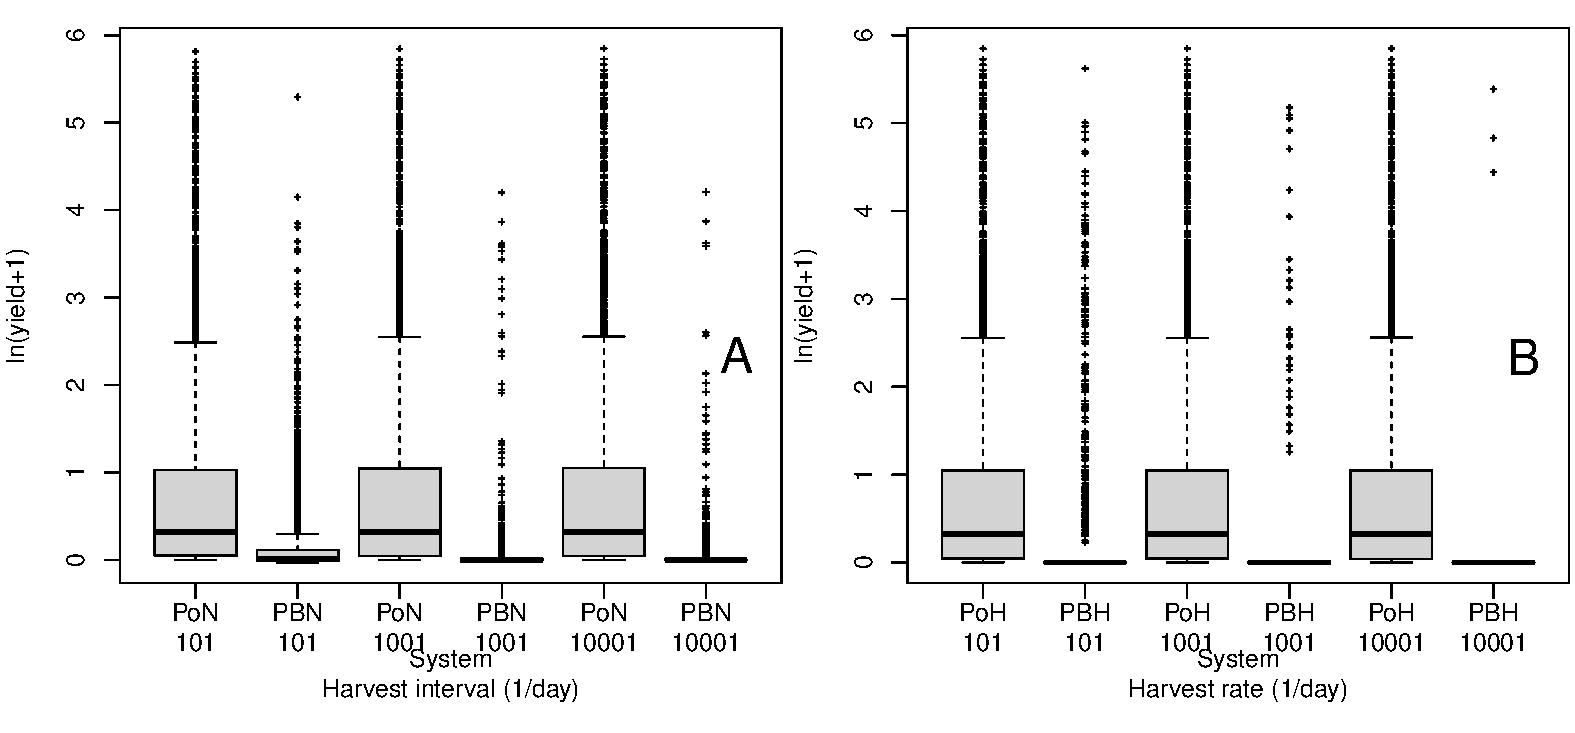
\includegraphics[width=\linewidth]{result/Harvest.pdf}
    \caption[Yield flux distribution by harvest mode]{Log distribution of yield for destructive (subplot A) and continuous (subplot B) harvest modes on selected harvest interval/rates.  For both subplots, pairwise Wilcox test showed significance between phytoplankton-only (\PoH/\PoN) and coexistence (\PBH/\PBN) systems (p $\ll$ 0.01), between harvest rates/intervals within the group of coexistence systems (p $\ll$ 0.01) but not phytoplankton-only systems (p $>$ 0.1).}
    \label{f:ydByHarv}
\end{figure}

\begin{figure}[H]
    \centering
    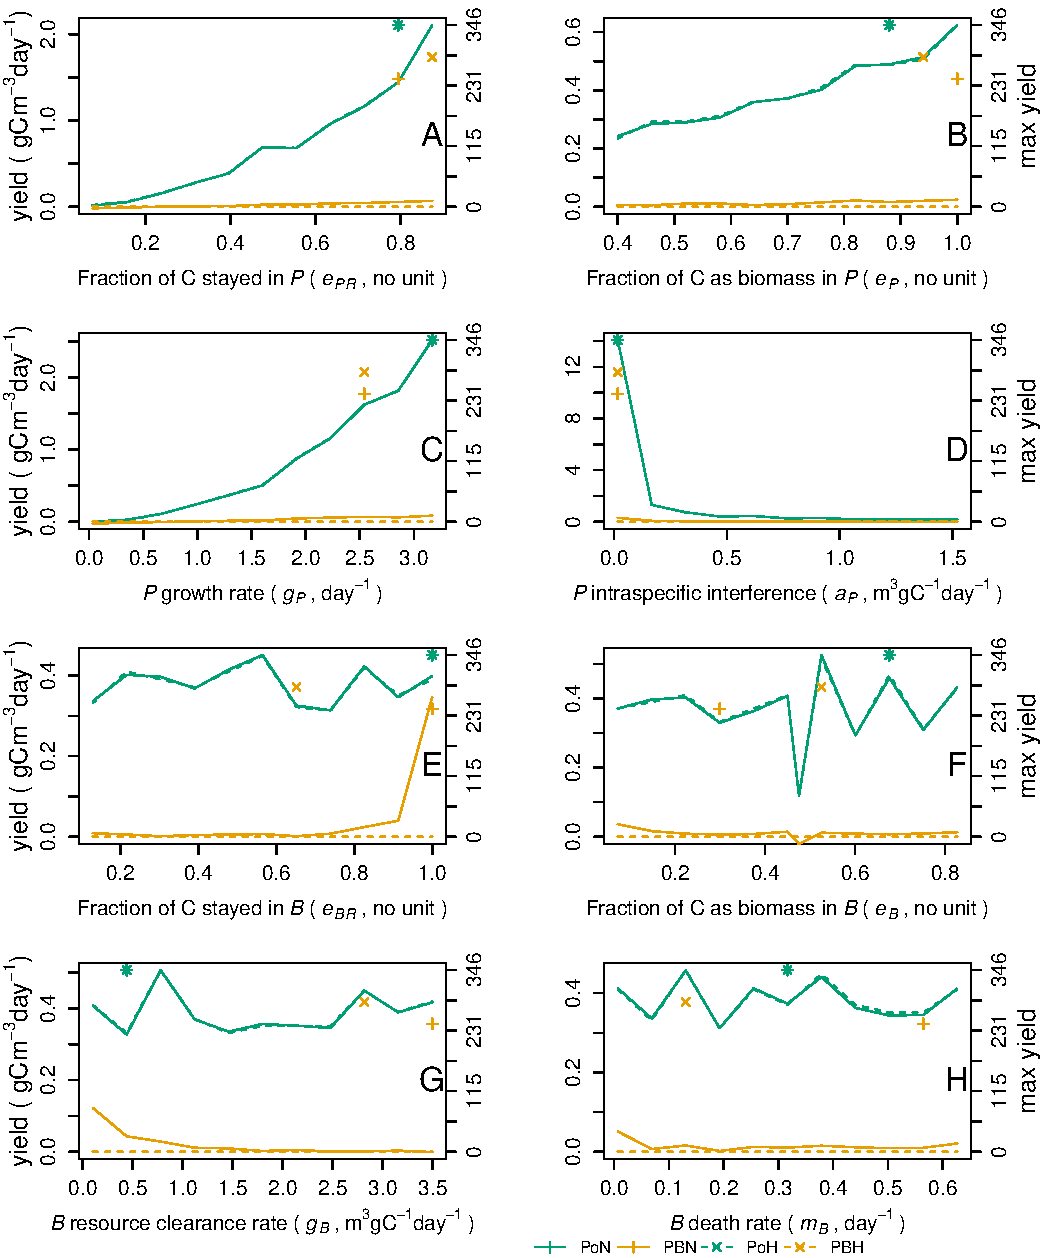
\includegraphics[width=\linewidth]{result/yieldFlux.pdf}
    \caption[Yield flux median in biological parameter space]{Log yield flux median (primary axis) and the maximum yield scenario (secondary axis) along respective parameter ranges under a standardised temperature range of \temp.  Each system had an LHS sample size of 1.1 million.  Pairwise Wilcox test showed significance (p $\ll$ 0.01) between all systems.}
    \label{f:ydByPara}
\end{figure}

\end{document}